% !TEX root =  ../report.tex

\section{Introduction}
%The introduction should provide content for the report, discuss relevant background material and state the main aims of the work. Clearly establishing the aims of the work is important for this coursework, since you have a great deal of freedom in what you will seek to achieve.

In the field of High Performance Computing (HPC), computers with processing power tens or hundreds of times greater than conventially available machines are used to solve (or appoximate solutions to) problems that would otherwise take an unwarrantable amount of time. Such computers have been required for some time to make use of a large degree of parallelism in order to complete with reasonable runtime: dividing work into independant subsections which can be executed simultaneously.
\par Many paradigms for executing parallel workloads have emerged over time: including vector instructions (SIMD), many and multi-core CPUs, clusters of interconnected computers, and General Purpose Graphical Processing Units (GPGPUs). Hardware which was originally specilised for graphical shader calculations through it's very high number of processing units, allows carrying out the same operation across a very large amount of data in parallel. This harware has been adapted in GPGPUs to perform non-specific operations that would normally have been done by the CPU.
\par
There is always space for further benefit to be gained, and even small gains in runtime can have large impact on workload that take hours or days to complete. This report details an investigation into applying a new optimisation to the CUDA code generation library subsection of OP2, and secondarily benchmarking what performance gain if any it is able to provide. The optimisation is named "Just-In-Time Compilation" for its similarities to a comparable process often performed by compilers when runtime efficiency is desired.

\subsection{Background Work}
\label{sec:bgwork}
The OP2 library is an Open Source Domain Specific Langauge (DSL) which provides a high level abstraction for describing physics problems which can be abstracted to an Unstructured Mesh.
A large proportion of HPC workloads involve approximating Partial Differential Equations (PDEs) to simulate complex interactions in physics problems, for example the Navier-Stokes equations for computational fluid dynamics, prediciting weather patterns, or computational electro-magnetics. It is usually necessary to discretise such problems across some form of mesh, either structured (regular) or unstructured.

\begin{figure}[h!]
  \begin{minipage}{.5\textwidth}
    \centering
    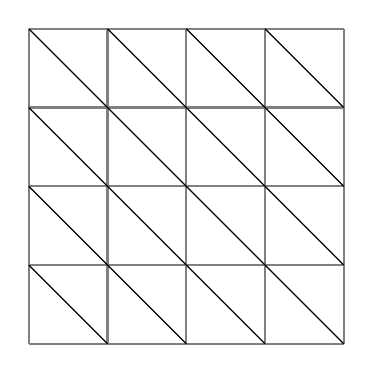
\begin{tikzpicture}
      \draw[step=1cm,gray,thick]
      (0,0) grid (4,4);

      \foreach \x in {0,...,3}{
        \draw (\x, 0) -- (0, \x) ;
        \draw (\x, 4) -- (4, \x) ;
      }

    \end{tikzpicture}
    \caption{Tri-Structured Mesh}
    \label{fig:struct}
  \end{minipage}
  \begin{minipage}{.5\textwidth}
    \centering
    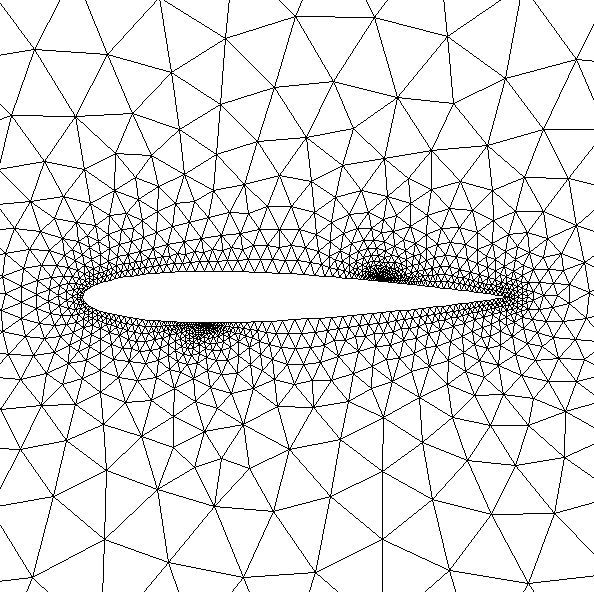
\includegraphics[width=.55\textwidth]{umesh}
    \caption{Airfoil Tri-Unstructed Mesh}
    \label{fig:umesh}
  \end{minipage}
\end{figure}
\par
Unstructed Meshes, such as Figure \ref{fig:umesh}, use connectivity information to specify the mesh topology. The position of elements is highly arbritrary, unlike structured meshes where elements follow a regular pattern (Figure \ref{fig:struct}). A particular simulation might, for example, be approximating the velocity of a fluid in each cell based on the cells around it.

\subsection{Motivations}
The idea for this project was provided by my supervisor, Dr Gihan Mudalige - an Associate Proffesor in the University of Warwick Computer Science Department. It was pulled from the pool of uncompleted features for the OP2 project, and I selected it as it aligned with my interest in High Performance Computing, and similar experience with optimising exisiting codes.
\par
Since OP2 is Open Source and freely available, the implementation I produce will become part of the library, allowing future contributors to build on my work. The project also allows me the opportunity to operate on a large codebase, where most university work is done largely within the confines of one's own code.
